\section{eo\-Segment\-Crossover$<$ EOT $>$ Class Template Reference}
\label{classeo_segment_crossover}\index{eoSegmentCrossover@{eoSegmentCrossover}}
eo\-Segment\-Crossover --$>$ uniform choice in segment == arithmetical with same value along all coordinates  


{\tt \#include $<$Tutorial/eo\-Real\-Op.h$>$}

Inheritance diagram for eo\-Segment\-Crossover$<$ EOT $>$::\begin{figure}[H]
\begin{center}
\leavevmode
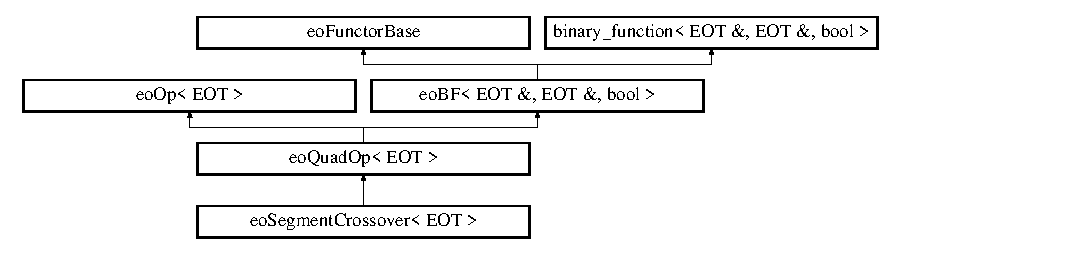
\includegraphics[height=2.96296cm]{classeo_segment_crossover}
\end{center}
\end{figure}
\subsection*{Public Member Functions}
\begin{CompactItemize}
\item 
{\bf eo\-Segment\-Crossover} (const double \&\_\-alpha=0.0)
\begin{CompactList}\small\item\em (Default) Constructor. \item\end{CompactList}\item 
{\bf eo\-Segment\-Crossover} ({\bf eo\-Real\-Vector\-Bounds} \&\_\-bounds, const double \&\_\-alpha=0.0)
\begin{CompactList}\small\item\em Constructor with bounds. \item\end{CompactList}\item 
virtual std::string {\bf class\-Name} () const \label{classeo_segment_crossover_a2}

\begin{CompactList}\small\item\em The class name. \item\end{CompactList}\item 
bool {\bf operator()} ({\bf EOT} \&\_\-eo1, {\bf EOT} \&\_\-eo2)
\begin{CompactList}\small\item\em segment crossover - modifies both parents \item\end{CompactList}\end{CompactItemize}
\subsection*{Protected Attributes}
\begin{CompactItemize}
\item 
{\bf eo\-Real\-Vector\-Bounds} \& {\bf bounds}\label{classeo_segment_crossover_p0}

\item 
double {\bf alpha}\label{classeo_segment_crossover_p1}

\item 
double {\bf range}\label{classeo_segment_crossover_p2}

\end{CompactItemize}


\subsection{Detailed Description}
\subsubsection*{template$<$class EOT$>$ class eo\-Segment\-Crossover$<$ EOT $>$}

eo\-Segment\-Crossover --$>$ uniform choice in segment == arithmetical with same value along all coordinates 



Definition at line 247 of file eo\-Real\-Op.h.

\subsection{Constructor \& Destructor Documentation}
\index{eoSegmentCrossover@{eo\-Segment\-Crossover}!eoSegmentCrossover@{eoSegmentCrossover}}
\index{eoSegmentCrossover@{eoSegmentCrossover}!eoSegmentCrossover@{eo\-Segment\-Crossover}}
\subsubsection{\setlength{\rightskip}{0pt plus 5cm}template$<$class EOT$>$ {\bf eo\-Segment\-Crossover}$<$ {\bf EOT} $>$::{\bf eo\-Segment\-Crossover} (const double \& {\em \_\-alpha} = {\tt 0.0})\hspace{0.3cm}{\tt  [inline]}}\label{classeo_segment_crossover_a0}


(Default) Constructor. 

The bounds are initialized with the global object that says: no bounds.

\begin{Desc}
\item[Parameters:]
\begin{description}
\item[{\em \_\-alpha\-Min}]the amount of exploration OUTSIDE the parents as in BLX-alpha notation (Eshelman and Schaffer) 0 == contractive application Must be positive \end{description}
\end{Desc}


Definition at line 259 of file eo\-Real\-Op.h.\index{eoSegmentCrossover@{eo\-Segment\-Crossover}!eoSegmentCrossover@{eoSegmentCrossover}}
\index{eoSegmentCrossover@{eoSegmentCrossover}!eoSegmentCrossover@{eo\-Segment\-Crossover}}
\subsubsection{\setlength{\rightskip}{0pt plus 5cm}template$<$class EOT$>$ {\bf eo\-Segment\-Crossover}$<$ {\bf EOT} $>$::{\bf eo\-Segment\-Crossover} ({\bf eo\-Real\-Vector\-Bounds} \& {\em \_\-bounds}, const double \& {\em \_\-alpha} = {\tt 0.0})\hspace{0.3cm}{\tt  [inline]}}\label{classeo_segment_crossover_a1}


Constructor with bounds. 

\begin{Desc}
\item[Parameters:]
\begin{description}
\item[{\em \_\-bounds}]an {\bf eo\-Real\-Vector\-Bounds}{\rm (p.\,\pageref{classeo_real_vector_bounds})} that contains the bounds \item[{\em \_\-alpha\-Min}]the amount of exploration OUTSIDE the parents as in BLX-alpha notation (Eshelman and Schaffer) 0 == contractive application Must be positive \end{description}
\end{Desc}


Definition at line 270 of file eo\-Real\-Op.h.

\subsection{Member Function Documentation}
\index{eoSegmentCrossover@{eo\-Segment\-Crossover}!operator()@{operator()}}
\index{operator()@{operator()}!eoSegmentCrossover@{eo\-Segment\-Crossover}}
\subsubsection{\setlength{\rightskip}{0pt plus 5cm}template$<$class EOT$>$ bool {\bf eo\-Segment\-Crossover}$<$ {\bf EOT} $>$::operator() ({\bf EOT} \& {\em \_\-eo1}, {\bf EOT} \& {\em \_\-eo2})\hspace{0.3cm}{\tt  [inline, virtual]}}\label{classeo_segment_crossover_a3}


segment crossover - modifies both parents 

\begin{Desc}
\item[Parameters:]
\begin{description}
\item[{\em \_\-eo1}]The first parent \item[{\em \_\-eo2}]The first parent \end{description}
\end{Desc}


Implements {\bf eo\-BF$<$ EOT \&, EOT \&, bool $>$} {\rm (p.\,\pageref{classeo_b_f_a1})}.

Definition at line 282 of file eo\-Real\-Op.h.

References eo\-Real\-Base\-Vector\-Bounds::is\-Max\-Bounded(), eo\-Real\-Base\-Vector\-Bounds::is\-Min\-Bounded(), eo\-Real\-Base\-Vector\-Bounds::maximum(), eo\-Real\-Base\-Vector\-Bounds::minimum(), and eo\-Rng::uniform().

The documentation for this class was generated from the following file:\begin{CompactItemize}
\item 
eo\-Real\-Op.h\end{CompactItemize}
